
\section{Experiment 1: Pull request evaluation}\label{sec:pull_request_eval}
In this section, the first evaluation about pull requests  related to data clump refactoring is discussed. 

To ascertain the quality of refactoring, human feedback is essential \cite{search_based_refactoring}. While there are metrics to evaluate whether a given refactoring is useful, the metrics do not always align with the viewpoints of developers. 

 For example, the \textit{DataClumpDoctor} tool might identify data clumps that not all developers would agree are problematic. Discrepancies might arise over the minimal number of data clump items (three in this master's thesis). Additionally, developers who are  familiar with the projects's structure may more accurately judge  whether a group of variables  is worth refactoring. In some cases, they have written the method or class themselves and have introduced the data clump on purpose. One reason for this decision could be that they were unable to find a proper name for the extracted class, or the disadvantages discussed in section \ref{sec:data_clump_not_refactor} outweigh the advantages of removing data clumps.

Even if developers see that refactoring a data clumps could be helpful, there could be arguments against refactoring them. These reasons include the points  discussed in section \ref{sec:data_clump_not_refactor}. However, there could also be other reasons that apply to code smells in generals. For instance, developers might combine refactoring with the introduction of new features, rather than refactor solely for its own sake. 

As a result, collecting  the opinions and insights of developers on whether data clump refactoring is justified and can be performed by a \ac{LLM}  forms the foundation of this evaluation.





\subsection{Methodology}

Figure \ref{fig:flowchart_expA} shows the general methodology of the first experiment. 
In this experiment, GitHub projects were selected to refactor a single selected data clump via a pull request and feedback was collected from contributors of the projects to ascertain the refactoring quality of ChatGPT. 


\begin{figure}[ht!]
    \centering
    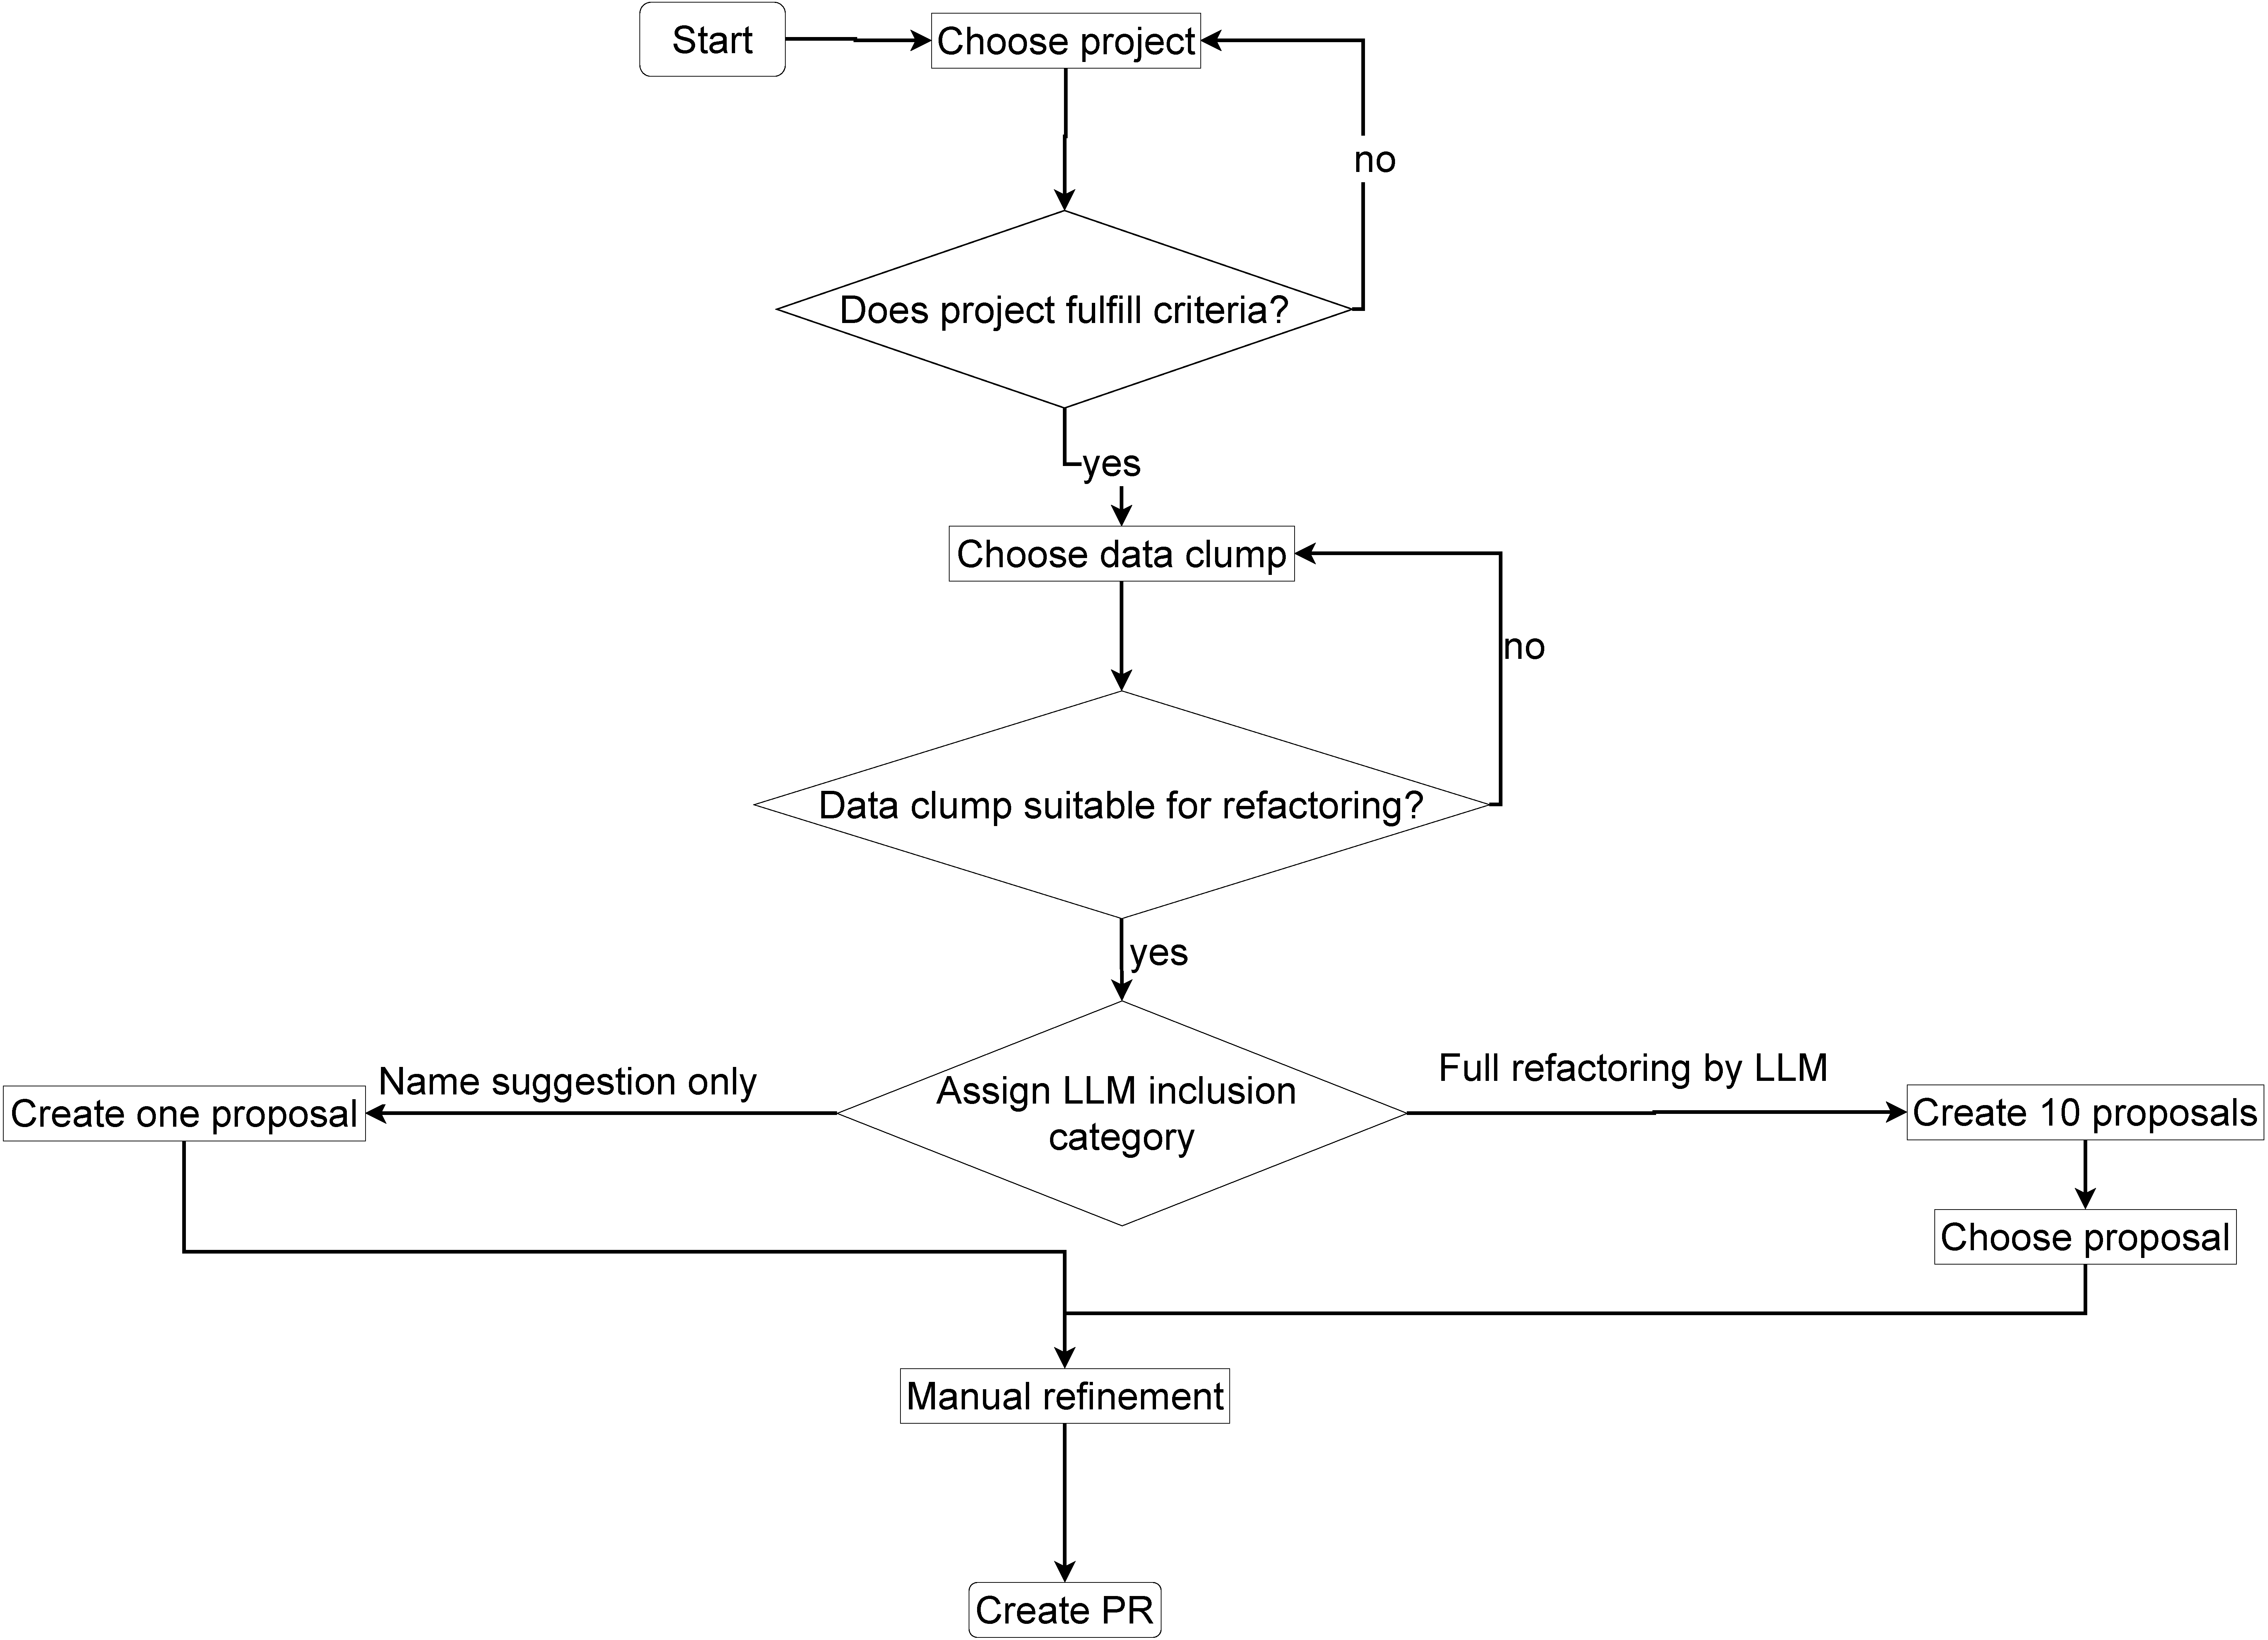
\includegraphics[width=1\columnwidth]{figures/chapter5/flowchart_expA.drawio.pdf}
    \caption{Methodology of the first experiment}
    \label{fig:flowchart_expA}
\end{figure}

\subsubsection{GitHub project selection}\label{sec:github_projects}

To facilitate the evaluation, GitHub projects are selected to be analyzed in the first experiment. 


The projects were selected from the trending page of GitHub. This page list GitHub projects that have gained significant attention over a specific  period. While the exact criteria for this listing is not disclosed, popular indicators include higher-than-average forks and stars.

To ensure a sufficient number of data clumps, only larger projects were considered. This increases heuristically the chance of having a higher number of data clumps, and also the chance of getting more developers to respond to the survey as larger projects tend to be maintained by more people. 

Since active participation of developers was necessary for the survey to work, only process with recent activity are selected. Only if pull requests are frequently considered and closed (which does not necessarily mean that they are merged), the project was considered active enough. 

In addition, the project had to be able to build without flaws. This ensures that the eventual refactoring can be evaluated smoothly. If the project did not compile properly or tests were failing, it became more difficult to determine whether these errors were caused by a refactoring or whether they existed from the beginning. This would be an obstacle to the manual refinement step.

%As a result, it was beneficial to make sure that these projects do build correctly. This can be checked by executing \textit{mvn clean package} or \textit{gradle clean build} (depending on the build system) as these commands usually run all required tests.

Hence, each selected project must comply with the following criteria:
\begin{enumerate}
    \item The project contains at least  10,000 \ac{LOC} of Java
        \item The project  has at least 100 stars
\item Any pull requests have been merged in the last 30 days
\item The project compiles and all tests run flawlessly.
\end{enumerate}


The total number of projects and hence pull requests was not predetermined at the beginning of the experiment. The goal was to create as many pull requests as possible. 


\subsubsection{Guidelines for selecting data clumps}

For each selected project, one data clump was chosen. To initialize this data clump selection process, the metrics described in section \ref{sec:data_clump_filtering} were combined. These metrics include the occurrence, size, and affected files metric. The top ten most-scored data clumps were manually reviewed to determine a data clump for refactoring. The selection process was supported by:
\begin{itemize}
\item A proposal by ChatGPT. 
    \item Any filter discussed in section \ref{sec:data_clump_filtering} would trigger (e.~g. abstract class, generics, annotations).
    \item The data clump items shared a common domain such that extracting a class would be useful. 
    \item The project was a library used by other programs so that refactoring of public or protected components should be carefully scrutinized. 
\end{itemize}

\subsubsection{LLM inclusion category}

After considering all of these criteria, one final data clump was selected.
After a data clump is selected, the next step was to assign the project to one of two categories to determine the extent \acs{LLM} were used to find and refactor data clumps. 



In the first category, ChatGPT performs the refactoring alone. Because transmitting whole GitHub projects would infeasible, the \textit{DataClumpDoctor} was used to detect the previously selected data clump and obtain all locations of interests. A margin of 5 was used so that 5 lines below and 5 lines above each location of interest were transmitted. 

Then, ChatGPT was instructed to refactor the data clump in the provided locations of interest. This instruction was repeated at least ten times, in each time the context of ChatGPT was cleared so it did not know its previous answers. 

From these ten proposals, one proposal was chosen that describes refactoring data clumps most accurately. For instance, the extracted class is valid, most usages of the data clump items are updated and all method signatures are refactored (if applicable). Generating multiple proposals is necessary because not every proposal would be correct. 



The second approach for refactoring was via IntelliJ. In this case, ChatGPT only suggests a suitable name for the extracted class but is otherwise not involved in the refactoring. Instead, the \ac{PSI} performs all refactoring in the manner described in section  \ref{sec:intellij_refactoring}. This results in a very consistent refactoring without any creativity. Hence, this refactoring needed to be executed only once and the first proposal can be selected immediately. 

\subsubsection{Manual refinement}

After selecting a proposal, the proposal is applied and saved on a separate branch.
Afterwards, the proposal might not be fully correct. For instance, there might be  none-updated method calls, missing semicolons etc. An additional problem occurs if code style tools like \textit{SpotBugs} or \textit{Checkstyle} are employed. If the refactoring by the \ac{LLM} does not conform to the required codestyle, the code might not compile because the developers of the project force a certain style. Therefore, a manual correction step is performed. The project is  manually changed in such a way that it fully compiles. However, no creative refactoring is performed. For instance, if one part of the source code was not refactored, it was refactored like another part regardless of whether another refactoring might have made more sense. This reduces human intervention to a minimum and ensures that the creative part of the refactoring is done by the \ac{LLM}. 

\subsubsection{\ac{PR} creation}
As soon as this manual refactoring finished and the program compiles, the changes were squashed into one commit and a pull request was created in the respective repository.

 A pull request is a proposal by a contributor to change some parts of the source code in a GitHub project. These changes can relate to fixing bugs, introducing new features or refactoring the code base. The proposals can be discussed and amended so that the proposal can be improved. By using continuous integration and continuous deployment, the changes can be tested automatically. Only if the changes are acceptable to an integrator (e.~g. the owner of the GitHub project), the changes are merged into the project. If not, the pull request can be closed without further consequences. \cite{pr_decisions}

In the pull request of the experiment, the maintainers were described the purpose of this pull request and  the definition of data clumps used in this master's thesis. They were asked to give feedback by filling out a feedback form or by giving feedback via GitHub comments under the respective pull request. It was explicitly stressed that rejecting the pull request would not be perceived negatively. The full text of the pull request can be found in appendix \ref{app:pr_text}.

\subsubsection{Feedback survey}\label{sec:feedback_survey}

Feedback was collected from two sources that were available on each pull request. 

One  natural way of providing feedback over GitHub is via comments. These comment can be review comments that address specific parts of the code, or general comments unrelated to any code that addresses the pull request as a whole. \cite{10.1145/3597208}. Therefore it is an important source of determining the acceptance of the proposed refactoring. However, since the comments are natural texts, the evaluation is more challenging.


On the other hand, surveys commonly use the Likert scale, which presents statements and asks respondents to choose a response from discrete attitude categories. \cite{HARPE2015836}
For instance, a statement might be \enquote{Data clumps are a code smell that should be fixed} and a respondent could choose between \enquote{Agree}, \enquote{Neutral} or \enquote{Disagree} for this statement. 


The topics of the survey  ranged from the usability of \acp{LLM} in software engineering, to the quality of the proposed refactoring, and the experience of the respondents. 


Details about the survey can be found in appendix \ref{app:pr_survey}


\subsubsection{Evaluation metrics}

For the evaluation, the following metrics are used:
\begin{itemize}

    \item  How many PRs are merged or rejected.
    \item The numerical value of the Likert scale.
    \item Topics mentioned in the comments that are either positive or negative. For instance, a comment might mention that the readability is improved or worsened by a refactoring. The occurrence of these topics can be counted.   Table \ref{tbl:feedback_categories} explains the most important feedback categories. 

\end{itemize}

By grouping the pull requests into categories (e.~g. by refactoring method, data clump type etc.), these metrics can be used to gather hindsight into the acceptance of \ac{LLM}-assisted refactoring. 

To evaluate this experiment, the null hypothesis \enquote{Developers do not accept data clump refactoring via \ac{LLM}} is presumed. This null hypothesis is rejected if \textbf{all} of the following conditions are met:

\begin{enumerate}
    \item At least 20~\% of the pull requests are merged
    \item The median Likert score for each of the survey questions is at least \enquote{Agree} (or 3 numerically)
\end{enumerate}

The first criteria takes into account that even good pull requests can be rejected for any reason so that a high threshold would not be helpful. The second criteria measures the acceptance of the PR. The feedback via text comments is left out as it would be difficult to describe a criteria by which the null hypothesis might be rejected.

Only if the developers generally agree with the changes by the pull request, the null hypothesis can be rejected with confidence. 


\begin{table}
\begin{tabular}{p{4cm}|p{10cm}}
	Comment & Description\\\hline
	\textit{Refactoring not worth it} & The refactoring does not provide enough advantages to justify it\\\hline
	\textit{Readability} & The readability of the source code is reduced \\\hline
	\textit{Not enough} & While the refactoring could be a good idea, more changes should be performed to make the refactoring more useful \\\hline
	\textit{Intentional design choice} & The duplication of variables is warranted so that changes are unnecessary \\\hline
	\textit{Style adaption} & The refactored code does not fit into the rest of the code as it violates style guidelines. \\\hline
	\textit{Complexity} & The refactoring introduces more complexity\\\hline
	\textit{Semantic changes} &  The refactoring changes the semantic of the code\\\hline
	\textit{Performance}& The performance implications of the refactoring are too grave \\\hline
	%\textit{Java record better} & The extracted class suggested by the refactoring could be converted into a Java record \\\hline
	%\textit{Extracted class should not be public} & Instead of creating a new file for an extracted class, it should be located inside another class and does not need to be public \\\hline
	
\end{tabular}
\caption{Feedback categories explained}
\label{tbl:feedback_categories}
\end{table} 




\subsubsection{Ethical consideration}
As this survey contains interaction with human-beings, a small analysis on the ethical implications is conducted. Several precautions are undertaken to address any possible ethical concern. 

First of all, full transparency is provided  with regard to the pull request. The pull request message explicitly states the purpose of the \ac{PR} as a part of a scientific project. Also the use of an \ac{LLM} is explicitly stressed so that no misunderstanding can occur. However, the participants are not aware of the extent \acp{LLM} have been used and do not know which model was used. Such details have however been revealed during discussion of the \ac{PR} if further feedback from new participants was unlikely.

Additionally, the requests were not sent en masse but after careful consideration. Only if it is thought that a pull request does compile, passes all unit tests and otherwise does not have major issues, the pull request is submitted. Of course, mistakes can happen so that this approach cannot guarantee hundred percent fault-free code. Since many projects needs to be considered, the extensive knowledge of the software project, which a regular contributor has, is missing, so that the chance of faults is higher. Nevertheless, pull requests can be created by anyone and the review process by continuous integration and deployment tools and human beings is a safeguard to limit the risk of faulty code added to the code base. 

Last but not least, it was attempted to minimize the burden on the reviewers. For instance, data clumps affecting a significant number of files were not refactored. Also only one pull request per project was created, thereby minimizing the chance that a participant might review multiple pull requests. 

At one instance, an ethical complaint was filed because of the use of \acp{LLM} and the perceived spamming of pull requests. This complaint was however dismissed by the responsible organizations of the University of Osnabrück.


\subsection{Results}

At the conclusion of this experiment, pull requests to 40 projects were submitted. Of those 40 projects,  feedback for 31 projects could be obtained. In the remaining 9 cases, either the pull request is still open, was closed without meaningful feedback or merged without meaningful feedback. In 8 cases, the pull request was eventually merged which indicates a acceptance rate of twenty percent. 

In 7 projects, feedback was provided via the survey. 8 comments were received via the survey which means that for one project the survey was filled out twice. Figure \ref{fig:boxplot_survey} shows the result of the evaluation if only the Likert scores are considered. 

The box plot shows that developers have a weak tendency to consider data clumps as a code smell worthy to fix as the median is about 2.5 (neutral to agree). Since the lower whisker shows a value of 1, it can be assumed that there is some disagreement about this code smell.

The statement that \acp{LLM} are useful receives more agreement. There is one outlier that has a neutral altitude whereas all other Likert values shows agreement or strong agreement. 

There is significant opposition to the claim that the proposed refactoring improves the source code. The median lies at 1 which indicates disagreement. 

With regard to the preservation of functionality, the respondents generally agree that the functionality is remains as before. One outlier exists. In that particular case, the handling of the \textit{NonNull} annotation is not preserved which the respondent sees as a disadvantage. 

As significant variance exists for the claim of the suitability of the chosen name for the extracted class. While the median is at 3, there is a wide range of different answers to this statement which indicate that the selected names are not always liked. 

On the other hand, there is less opposition for the location of the new class although the outlier show that the selection of the location still poses some challenges. 

As a result, while the first rejection condition of the null hypothesis is met, the second fails. Therefore, the null hypothesis fails to reject. This means that the first RQ \enquote{Do developers accept data clump refactoring via ChatGPT?} cannot be answered positively.

\bigskip
\begin{figure}
    \centering
    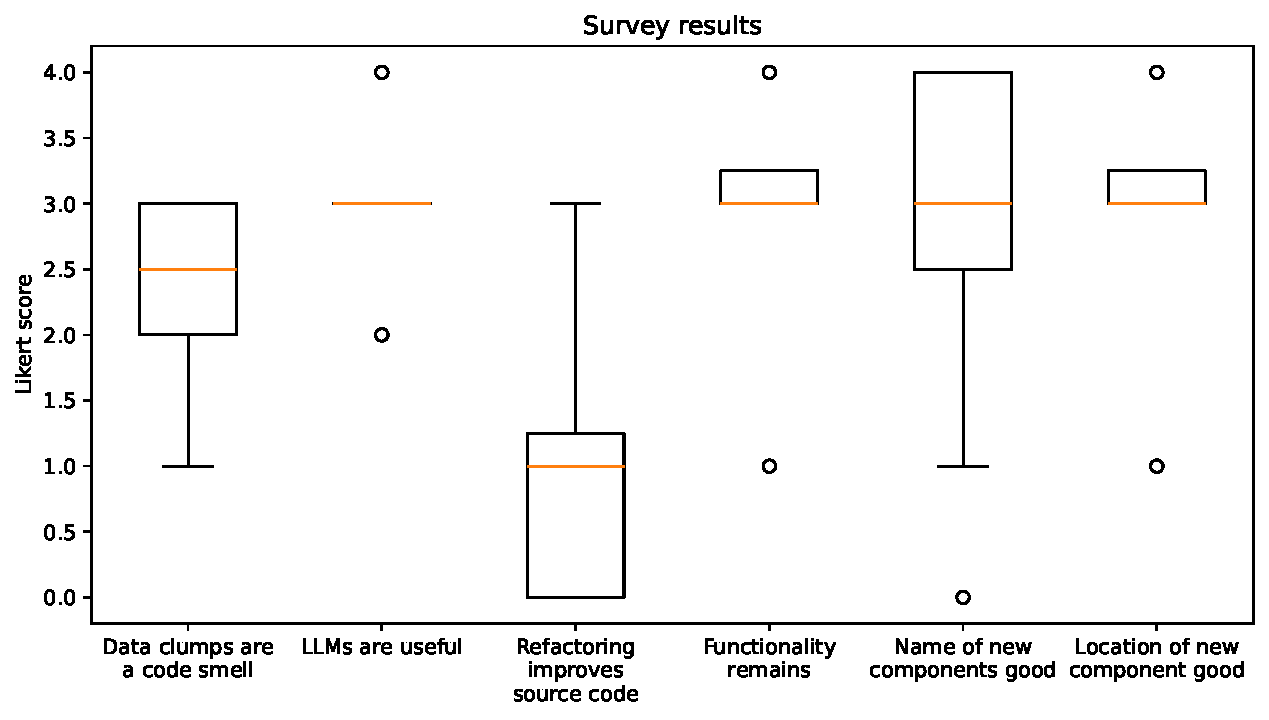
\includegraphics[width=\columnwidth]{figures/chapter5/survey_results.pdf}
    \caption{Boxplot of Likert score from survey}
    \label{fig:boxplot_survey}
\end{figure}


The textual feedback contains further hindsight on why the refactoring was perceived more negatively. In five instances, the reviewers perceived an increase of complexity. In 10 instances, there were concerns about the readability. Also, performance concerns were common as the refactoring entailed creating new instances. This criticism was shared five times. Another argument that was made 10 times is that the refactoring was not worth it as the developers see no obvious benefit in refactoring this data clump. In two cases, the developers cited legal reasons as a ground for rejection which shows that these issues are not fully resolved.

The difference of the feedback between the traditional refactoring and the \ac{LLM}-driven refactoring is slim. However, there are noteworthy observations. For instance, the traditional approach receives four instances where the maintainers are dissatisfied with the style adaptation of  the code. This means that the refactored code did not fit into the rest of the code. This point was not risen for the fully \ac{LLM}-generated code. 

Also, in general, criticism about the code readability was raised more for the project refactored using the traditional approach than the \ac{LLM}-based approach. In former approach, the readability was mentioned seven times negatively, in the latter approach three times. On the other hand, the projects refactored with the traditional approach received three comments claiming the readability was improved, and only one such comment for the \ac{LLM}-based approach. 

Comparing the refactoring of fields-to-fields to parameters-to-parameters data clump, there are also some differences. The readability of refactored fields-to-fields data clump was  scored more negatively than that of parameters-to-parameters data clump. Also the adoption of the code to the style was criticized more if fields-to-fields data clump were refactored. Additionally, more meaningful comments were received for parameters-to-parameters data clump.

Noteworthy, the refactoring performed by the model had not always refactored an actual data clump as defined in section \ref{sec:data_clump_def}. In one case, a group of fields that only existed in one class but have a semantic relationship were extracted to a class. Nevertheless, this pull request was merged indicating that a close semantic connection of variables can warrant refactoring. However, in two other similar cases, the pull request was rejected. 

The occurrence of a data clump strongly influences the likelihood of a refactoring being merged. Refactorings that were not merged had a mean occurrence of 4.5, whereas those that were merged had a mean occurrence of 10.7

If one considers the size of the refactored data clump, there are also some patterns. For instance, the respondents believe that larger data clumps reduce the complexity. However, on the other hand, the readability of the refactored source code was higher if the data clump is smaller.

\subsection{Threats to validity}

The survey evaluation has some threats to its validity that should not be disregarded.

To begin with, the selection of GitHub projects was not completely unbiased. For instance, currently trending GitHub projects were chosen although it is not certain why they were popular. Therefore, the maintainers of the project might not be fully prepared to deal with associated surge in pull requests associated with trending projects. This can increase the chance that a pull request (even though reasonable and well-meant) is summarily rejected. \cite{10.1145/3366423.3380272}

Additionally, only projects that do build flawlessly were considered. Usually, this should be case for every project, but the reality differs. For instance, the operating system, the installed libraries, the Java version, and other components can have a significant impact on whether all unit tests complete without errors and the project builds.  While every effort was made to give each project a chance to compile, at some point, time constraints prevented endless consideration of a project. Hence, if even after testing on multiple system, reading the associated documentation, and testing multiple Java version, no fully functional build was achieved, the project was disregarded.

It is also important to consider the manual correction process, as it could introduce mistakes or bugs due to human error rather than errors from the \ac{LLM}. Feedback regarding these errors must be filtered out as they are not relevant. This manual correction process can also shift the quality of the refactoring upwards so that the respondent would rate the raw \ac{PR} more negatively. 


Additionally, the decision to accept or reject a pull request can depend on many factors. For instance, the current mood of participating developers can influence the rejection rate \cite{detecting_emotional}.

For larger project, bureaucracy was also a factor that prevented the creation of pull requests. For instance, some projects require that pull request must always relate to an existing issue so that the general idea can be discussed without providing source code. For usual contributors, this might be beneficial as they do not need to spend time on writing code that is rejected in the end because the developers do not like the general approach. For the purpose of this evaluation, the actual source generated is essential, so creating an issue first would be possible,  but more burdensome  and would not add much value. Nevertheless, the sole existence of such rules was not a criterion to filter out a project. 

Furthermore, using a survey with the Likert scale can lead to problems since such an analysis can have its flaws as it implies that the distance between response categories is constant. For example, it might be easier or harder to choose between \enquote{Strongly Disagree} and \enquote{Disagree} compared to \enquote{Strongly Agree} and \enquote{Agree} \cite{HARPE2015836}.

As the results show, participation in the survey is essential. Because only seven developers responded to the survey, the results can only be taken with a grain of salt. The small sample size also means that the interpretation of the median and other statistical metrics is less meaningful.

The decision on whether the \ac{LLM} performs the full refactoring or only suggests a suitable name was not randomized enough. After all refactoring proposals were submitted, it was found out that the average occurrence of the data clumps refactored was 9.64 for the name suggestion approach. If the model performed the full refactoring, the average occurrence was 1.95. This suggests a selection bias as the decision to assign an \ac{LLM} inclusion approach was done by the experimenter. Although the same number of projects were refactored by either approach, the selection bias was still present at the end. However, the impact of this bias on the results is difficult to estimate. 

\subsection{Discussion}

One main finding on the evaluation results is the importance of selecting suitable data clumps for refactoring. In many cases, the developers believe that the suggested refactoring is not worth it, makes the code harder to read or the performance implication are too negative. This shows that data clumps are a code smell where there is a wide disagreement on when refactoring is warranted and when not. because all tested projects have a multitude of different data clumps that have various sizes, affected files or included variables, it is very difficult to select a suitable data clump. Traditional metrics like the size or the occurrence seem to have only a partial influence on the acceptance of data clump refactoring. Instead, the relationship of the variables is more often a better indicator. Here, the model can be a great help as it does not necessarily rely on these common metrics. However, as it can be seen, the choice by the model is often not enough. Instead, the inherent knowledge of the contributors of a project is a major factor in  deciding whether refactoring is warranted. Only with information about the scope, goals, and issues of a project, it is possible to determine where refactoring is more likely to be warranted. Even with the help of \ac{LLM}, external contributions can hardly mitigate this lack of knowledge which explains many pull request rejections. 

The results also show that the concrete refactoring proposed needs further adjustment. For instance, using the traditional method generates source code that was perceived less readable. One reason for this could be that the traditional approach always use the same algorithm for refactoring data clumps. For instance, it always generates getters and setters, and cannot observe the code style used in other files. On the other hand, the code generated by the model is often not enough, requires human intervention to compile, and also does not offer enough potential to be accepted by developers. This indicates that further prompt engineering and quality control is needed to better utilize \acp{LLM} such as ChatGPT

Another highlighted issue is the legal implication of using \acp{LLM} which is a significant concern for open source developers. Because large language models derive their knowledge from a multitude of sources, cannot give these sources adequately and are relatively new, the developers are too cautious to integrate refactorings by \acp{LLM}. Even without knowing that a traditional approach was used for the actual refactoring, merely mentioning the use of LLMs led to rejections.  This indicates that the legal implications of these models are fundamental and need to be resolved before they can be accepted. 

The results show that surveys via GitHub pull request pose some challenges. Some pull requests are left unanswered, while others are closed without comments or the comment contains very general feedback and not helpful for evaluating the survey. Additionally, the tendency of developers to use GitHub for giving feedback  instead of the suggested survey platform complicates a solid analysis of the evaluation.

In summary, RQ 1 cannot be answered positively. Additionally, the use of \acp{LLM} entails many challenges that remain unresolved. The main problem is the selection of a suitable data clump for refactoring because many developers think that the chosen data clump should not be refactored. Here, additional information from the source code, the commit history or other code-related data must be integrated into the pipeline so that the model can make a better decision. Additionally, the manual refinement phase is very important as the code refactored by the model leads to a good direction but needs to be adapted in order to compile. 